\documentclass{article}
\usepackage{graphicx}
\usepackage[T1]{fontenc}
% LTeX: language=es
% LTeX: language=en
\usepackage[spanish]{babel}
\graphicspath{ {./resources/} }
\usepackage{float}
\usepackage{listings}
\usepackage{xcolor}

\definecolor{codegreen}{rgb}{0,0.6,0}
\definecolor{codegray}{rgb}{0.5,0.5,0.5}
\definecolor{codepurple}{rgb}{0.58,0,0.82}
\definecolor{backcolour}{rgb}{0.95,0.95,0.92}

\lstdefinestyle{mystyle}{
    backgroundcolor=\color{backcolour},   
    commentstyle=\color{codegreen},
    keywordstyle=\color{magenta},
    numberstyle=\tiny\color{codegray},
    stringstyle=\color{codepurple},
    basicstyle=\ttfamily\footnotesize,
    breakatwhitespace=false,         
    breaklines=true,                 
    captionpos=b,                    
    keepspaces=true,                 
    showspaces=false,                
    showstringspaces=false,
    showtabs=false,                  
    tabsize=2
}

\begin{document}

\section{Introducción}

La siguiente guía de instalación busca guiar al usuario en la configuración básica de un laboratorio de Oracle Real Application Clusters, esta guía no busca enseñarle al usuario a utilizar Linux, pero si buscara proporcionar un poco de contexto adicional sobre ciertos comandos de Unix. El laboratorio utiliza 3 máquinas virtuales, las cuales usaran Linux con distribuciones basadas en Ubuntu y RHEL, por otro lado el sistema operativo puede ser cualquiera de preferencia por el usuario, pero en este caso se usará Pop\_Os!, el cual se encuentra basado en Ubuntu.

\section{Configuración de Máquinas Virtuales}

El primer paso consiste en preparar nuestras máquinas virtuales para los nodos de Oracle DB, estos usarán Oracle Linux 7 con Oracle DB 19c, acá cada nodo tiene cuenta con los siguientes requerimientos.

\begin{itemize}
	\item 4 GB de memoria RAM.
	\item 100 GB de almacenamiento físico.
	\item 2 núcleos de procesamiento.
\end{itemize}

Empezando con la creación del primer nodo en este cluster sera llamado ``node1'', aparte de las especificaciones ya mencionadas es necesario crear 3 adaptadores de red:

\begin{itemize}
	\item ``Host-only Adapter'': Usado para conectar à la base de datos hacia otros aplicativos.
	\item ``Internal Network Adapter'': Usado por la red interna del clúster.
	\item ``Bridged Adapter'': Usado para conectarse hacia el internet, usando al sistema operativo huésped.
\end{itemize}

\begin{figure}[H]
	\begin{center}
		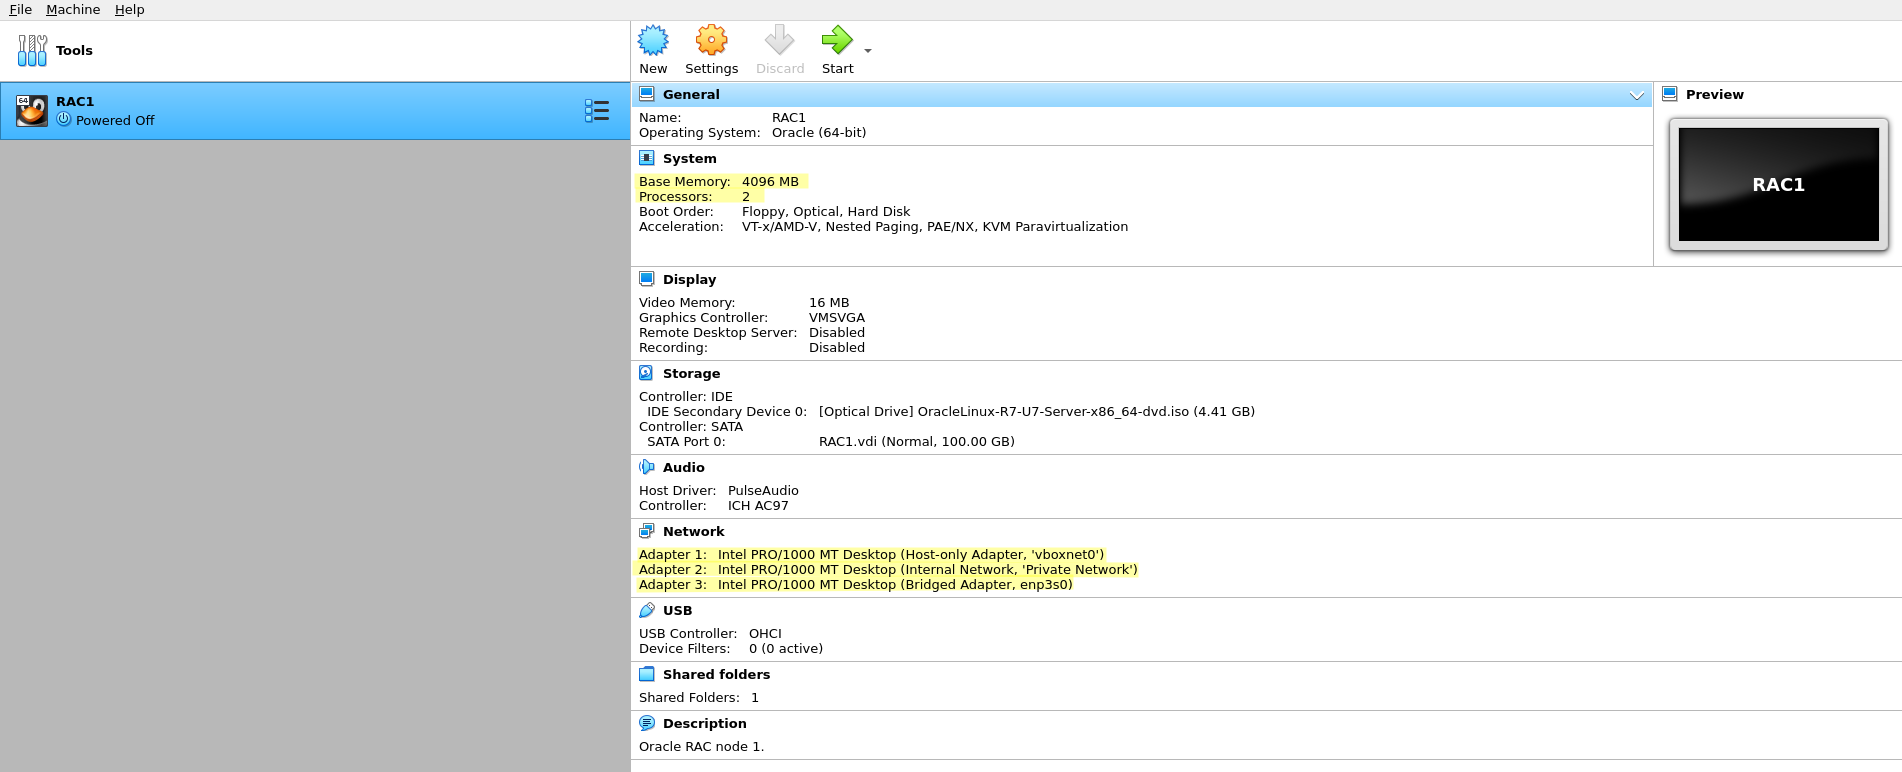
\includegraphics[width=0.95\textwidth]{vm_base.png}
	\end{center}
	\caption{Pantalla de inicio de Configuración de la Máquina Virtual}
\end{figure}

Al momento de iniciar la máquina virtual e insertar el archivo ISO con Oracle Linux 7, podemos empezar a configurar la instalación del sistema operativo. Acá iniciaremos con la configuración de partición del disco desde acá se selecciona ``Installation Destination'', en donde se puede ver el disco creado y las opciones de particiones, acá se seleccionará ``I will configure Partitioning''. Acá crearemos las siguientes particiones.

\begin{center}
	\begin{tabular}{ |c|c|c| }
		\hline
		\multicolumn{2}{|c|}{Lista de Particiones}    \\
		\hline
		Nombre de Partición & Capacidad               \\
		\hline
		/boot               & 2 GB de almacenamiento  \\
		/root               & 5 GB de almacenamiento  \\
		/ o root            & 50 GB de almacenamiento \\
		/swap               & 8 GB de almacenamiento  \\
		\hline
	\end{tabular}
\end{center}

Al volver al menú de inicio de nuestro instalador, se selecciona el software por instalar en nuestra nueva instalación, acá se selecciona la opción ``Software Selection'', acá se puede escoger entre varios ambientes, pero se seleccionará ``Server with GUI'' con los siguientes paquetes de software.

\begin{itemize}
	\item ``Hardware Monitoring Utilities''
	\item ``Large Systems Performance''
	\item ``Network file system client''
	\item ``Performance Tools''
	\item ``Compatibility Libraries''
	\item ``Development Tools''
\end{itemize}

Al volver al inicio del instalador se puede configurar las opciones de red en ``Network and Hostname'' para configurar los adaptadores de red instalados en las máquinas virtuales. 

Después de habilitar el primer adaptador de red, seleccione ``Configure'' y en la pestaña de ``ipv4'' se usara la dirección IP ``192.168.24.1/24'' con una salida de ``0.0.0.0''  manualmente.

\begin{figure}[H]
	\begin{center}
		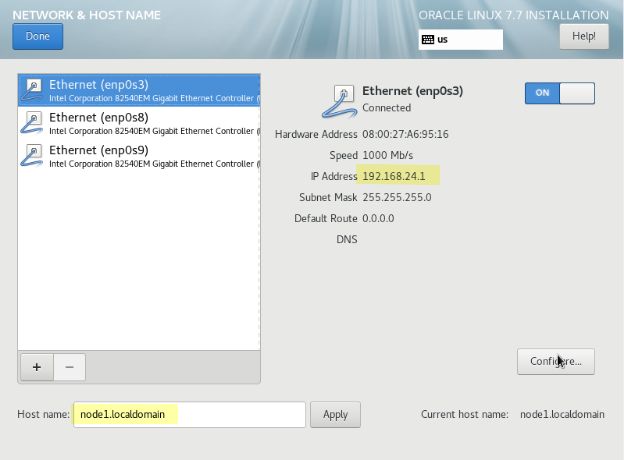
\includegraphics[width=0.95\textwidth]{vm_networking.png}
	\end{center}
	\caption{Configuración de Red de la Instalación de Oracle Linux}
\end{figure}

Se aplicará esta misma configuración manual en el siguiente adaptador disponible, pero esta vez con una dirección IP de ``192.168.10.1/24'' con una salida de ``0.0.0.0'', finalmente para el último adaptador habilitaremos direccionamiento automático con DHCP. Se puede continuar con la instalación del sistema operativo, en la siguiente pantalla podemos seleccionar una contraseña para el usuario ``sudo'', para este ejercicio se usará ``root'' como contraseña.

\section{Configuración del Sistema Operativo}

El siguiente paso consiste en preparar al sistema operativo para la instalación de los componentes de Oracle Grid y Oracle DB.

\subsection{Instalación de Paquetes}

Una vez en el ambiente de escritorio es necesario instalar software mediante el gestor de paquetes, en este caso esta distribución se encuentra basada en RHEL así que el gestor de paquete es yum.

\begin{lstlisting}[style=mystyle,language=bash]
	$ sudo yum update
	$ sudo yum install -y oracle-database-preinstall-19c.x86_64
	$ sudo yum install oracleasm-support
	$ sudo yum install bind* --skip-broken
\end{lstlisting}

\subsection{Configuración de Red}

Siguiente se configurara el archivo de hosts, según Verhage (2021) este archivo ubicado en \texttt{etc/host} se encarga de conectar direcciones ip con nombre de dominio.

\begin{lstlisting}[style=mystyle,language=bash]
	cat /etc/hosts
	127.0.0.1   	localhost
	::1         	localhost
	127.0.1.1   	pop-os.localdomain  	pop-os
\end{lstlisting}

En este caso, al visitar la dirección \texttt{127.0.0.1}, nuestro sistema operativo le indicará al navegador que debe de navegar hacia \texttt{localhost}. Para esto se puede abrir el editor de texto predeterminado del sistema operativo, gedit, o simplemente un editor de texto de consola, en este caso vim ya viene instalado. Aca se agregaran los siguientes cambios.

\begin{lstlisting}[style=mystyle,language=bash]
	# Default
	127.0.0.1   localhost localhost.localdomain localhost4 localhost4.localdomain4
	::1     	localhost localhost.localdomain localhost6 localhost6.localdomain6
	# Public
	192.168.24.1 node1.localdomain node1
	192.168.24.2 node2.localdomain node2
	# Private
	192.168.10.1 node-priv.localdomain node1-priv
	192.168.10.2 node2-priv.localdomain node2-priv
	# Virtual
	192.168.24.31 node1-vip.localdomain node1-vip
	192.168.24.32 node2-vip.localdomain node2-vip
	# SCAN
	192.168.24.41 node-scan.localdomain node-scan
	192.168.24.42 node-scan.localdomain node-scan
	192.168.24.43 node-scan.localdomain node-scan
\end{lstlisting}

Acá se esta mapeando los nombres de dominio con las redes a las cuales pertenece cada adaptador de red con el cual cuenta la máquina virtual, por esto mismo las direcciones proporcionadas se encuentran en la misma red.

\subsection{Configuración de Usuarios}

El uso de usuarios y grupos de usuarios permite restringir el acceso de estos sobre los distintos archivos en el sistema operativo, esto nos permitirá controlar su acceso sobre cualquier parte del sistema operativo, ya que la filosofía UNIX indica que ``todo es un archivo'' (ArchWiki, n.d.). Según la Wiki de ArchLinux (n.d) se puede crear a un nuevo usuario y grupo de usuarios con los siguientes comandos de consola:

\begin{lstlisting}[style=mystyle,language=bash]
	useradd John
	groupadd Accountants
\end{lstlisting}

Y para asignar entonces a un usuario a un grupo de usuarios se puede usar el siguiente comando de consola.

\begin{lstlisting}[style=mystyle,language=bash]
	useradd John
	groupadd Accountants
\end{lstlisting}

Con este contexto se puede crear a los grupos de usuarios requeridos para instalar la base de datos y configurar RAC.

\begin{lstlisting}[style=mystyle,language=bash]
	groupadd -g 54327 asmdba
	groupadd -g 54328 asmoper
	groupadd -g 54329 asmadmin
\end{lstlisting}

Aca la bandera \texttt{-g} permite asignar un identificador a cada grupo de usuario, podemos entonces verificar el contenido del archivo \texttt{/etc/group} para ver a los usuarios creados y sus grupos correspondientes.

\begin{lstlisting}[style=mystyle,language=bash]
	cat /etc/group | grep asm
	asmdba:x:54327:
	asmoper:x:54328:
	asmadmin:x:54329:
\end{lstlisting}

Estos nuevos usuarios tienen que pertenecer al grupo ya existente oracle, así que se va a modificar su grupo principal.

\begin{lstlisting}[style=mystyle,language=bash]
	usermod -G asmdba,asmoper,asmadmin oracle
\end{lstlisting}

Según Amoany (2021) podemos modificar la contraseña de un usuario con el comando \texttt{passwd}, en donde un usuario puede modificar únicamente su propia contraseña y un super-usuario puede modificar la contraseña de cualquier otro usuario en el sistema. Con este comando se modificara la contraseña para el usuario ya existente oracle.

\begin{lstlisting}[style=mystyle,language=bash]
	sudo passwd oracle
	[sudo] password for node1:
	Changing password for user oracle.
	New password:
	Retype new password:
	passwd: all authentication tokens updated successfully.
\end{lstlisting}

\end{document}
